\chapter{Complex Adaptive Systems}
\section{Self-Organization}
\section{Autonomic Computing}
\section{Distributed Intelligence}

\chapter{Designing Complex Systems' Software}
\section{Agents and \aclp{MAS}}

As software grows in complexity, 
traditional centralized architectures often become difficult 
to maintain, extend, and scale. 
%
Modern software systems are therefore characterized by autonomous and distributed components 
that cooperate to achieve common objectives. 
%
One way to design such components is to model them as \emph{computational agents}~\cite{WooldridgeJ99}.

As computational entities, agents are autonomous as they encapsulate their own \emph{control flow}~\cite{objag-jot1}.
%
Control-flow encapsulation is commonly referred to as \emph{computational} autonomy~\cite{artifacts-jaamas17},
and it is considered a necessary -- yet not sufficient -- pre-requisite for autonomy in software agents.

Computational agents are autonomous entities~\cite{OmiciniRV08}
situated in an environment that they can perceive and affect.
%
Unlike passive software components, 
agents exhibit autonomous behavior,
continuously perceiving their surroundings, 
reasoning about the current state of the system, 
and selecting appropriate actions to achieve their objectives.

A \ac{MAS} consists of multiple agents interacting within a shared environment.
%
While each agent pursues its own goals autonomously, 
they interact with one another to 
coordinate their actions fostering the achievement of shared goals.

Interaction among agents can occur either \emph{directly} or \emph{indirectly}.
%
Direct interaction relies on explicit communication between agents through message exchanges.
%
Indirect interaction, instead, takes place through modifications of the shared environment..
%
The latter mechanism is commonly referred to as \emph{stigmergy}~\cite{ch30-castelfranchifestschrift2012,HadeliVKB04}:
the actions performed by one agent alter the environment, and such alterations can subsequently be perceived by other agents, which adapt their behavior accordingly.

To support stigmergic coordination in software systems,
some \ac{MAS} technologies provide explicit and programmable abstractions for the environment~\cite{weyns2007aamas}.
%
In such cases,
the environment is not merely the execution context in which agents operate, 
but becomes an active component of the software system, 
containing shared information that agents can perceive and modify.
%
In this direction, 
some \ac{MAS} platforms provide dedicated abstractions, 
such as actions or artefacts, 
to support this kind of interactions~\cite{OmiciniRVCT04}.

Communication represents the most explicit form of interaction among agents, 
where information is exchanged by means of messages.
%
Message exchanges may be organised into structured conversations following well-established interaction patterns, 
commonly known as interaction protocols\footnotemark.
%
\footnotetext{FIPA Interaction Protocols, archived at
\url{https://archive.is/phy6v}}
%
Within an interaction protocol, 
each participating agent plays a specific role 
and is expected to exchange messages only at predefined stages 
of the conversation and according to the rules prescribed by the protocol.
%
% From a technological perspective,
% \ac{MAS} platforms must provide suitable message-passing mechanisms.
% Solutions range from simple in-process method invocations,
% limiting communication to agents executing within the same process,
% to distributed infrastructures relying on network protocols and middleware services such as brokers, message queues, or dedicated communication services, allowing agents executing on different machines to interact seamlessly.
%
In order to effectively communicate,
agents also require a common semantic interpretation of exchanged messages.
%
One way to do so,
is to rely on \acp{ACL}~\cite{kone2000kais},
namely high-level message formats enriched with metadata describing the intended meaning of each message~\cite{Chaib-draaD02}.
%
One of the best-known examples is \ac{KQML}~\cite{finin1994KQML},
which combines the role of message format and \ac{ACL},
with particular emphasis on knowledge exchange among agents.
%
Among its metadata,
the \emph{performative} specifies the communicative intention of the sender,
thus defining the semantic purpose of the message within the interaction protocol.
%
Derived from speech-act theory~\cite{traum1999speech},
performatives include actions such as informing another agent
(\texttt{tell}),
requesting the achievement of a goal
(\texttt{achieve}),
asking for information
(\texttt{askOne}, \texttt{askAll}),
or exchanging procedural knowledge
(\texttt{askHow}, \texttt{tellHow}).

\section{BDI}
\label{sec:bdi}

Among the several approaches for designing autonomous agents,
the \ac{BDI} definition is one interesting approach~\cite{RaoG95}.
%
\ac{BDI} systems represent a wide yet specific class of \acp{MAS},
where rational agents feature \emph{cognitive} abstractions.
%
Rather than describing agents exclusively in terms of inputs and outputs,
the \ac{BDI} architecture defines their behavior through explicit mental attitudes,
providing an abstraction of practical reasoning that closely resembles human decision making.
%
This abstraction was inspired by the work of the philosopher Michael Bratman,
which introduced the notions of
\emph{beliefs},
\emph{desires},
and
\emph{intentions}
to explain humans' practical reasoning~\cite{bratman1987intention}.
%
Later,
these ideas were formalized through modal logics~\cite{CohenL90}
and eventually inspired computational models for autonomous software agents.

\ac{BDI} characterizes agents in four fundamental abstractions~\cite{rao1991bdi}: 
\emph{beliefs}, \emph{desires}, \emph{intentions}, and \emph{plans}.

\paragraph{Beliefs}
Agents maintain a personal representation of the environment's state,
which is perceived by them during their execution.
%
Practically,
agents hold a set of beliefs,
also defined as a \emph{belief base},
which represents the agent's
\emph{epistemic} memory,
describing its knowledge about itself,
the environment,
and possibly other agents.
%
Beliefs represent the \emph{mental state} of the agent, 
which changes with the environment state over time.
%
In particular,
the mental state is made up of belief states, 
which represent an instance of the belief base held by the agent at a given time~\cite{KinnyGR96}.


\paragraph{Desires}
Each agent has a set of goals representing desirable states of the world that the agent
attempts to achieve,
test,
or maintain.
%
Desires are considered as the \emph{motivational} state of the agent.

\paragraph{Intentions}
Each agent hasa set of tasks to which it is currently committed,
namely the activities that it has decided to pursue.
%
Intentions serve to keep track of the progress towards the achievement of the agent's goals,
which happens by means of the execution of the corresponding intentions.

\paragraph{Plans}
Procedural descriptions that encode how intentions can be achieved under
specific circumstances,
thereby representing the agent's procedural knowledge.
%
Plans are selected for execution based on the agent's current beliefs and desires,
and, in order to be achieved,
they may require the execution of other plans.

These abstractions are not static,
but continuously evolve during the execution of the agent.
%
New perceptions obtained from the environment may introduce new beliefs,
invalidate obsolete ones,
or enrich the agent's knowledge.
%
Similarly,
agents may acquire beliefs through communication with other agents
or through the conclusions produced by their own reasoning process.
%
Changes in the environment may also affect the set of desires,
introducing new objectives or making existing ones no longer relevant.
%
Accordingly,
the agent continuously revises its intentions,
committing to new activities,
dropping obsolete ones,
or reconsidering previous commitments.

Committing to an intention means selecting one or more plans
capable of achieving the desired objective,
and executing them during the agent's lifecycle iterations.
%
Plans may involve the execution of actions affecting the environment,
the exchange of information with other agents,
or the generation of additional sub-goals,
whose accomplishment recursively activates further plans.

Finally,
agents may enrich their own procedural knowledge by acquiring new plans,
either as the result of internal reasoning
or through interactions with other agents.

One of the earliest and most influential implementations of the \ac{BDI}
architecture is \agentspeak{}~\cite{rao1996maamaw}, a programming language based on the Procedural Reasoning System (PRS)~\cite{georgeff1987reactive}.
%
The abstractions introduced \agentspeak{} provide the conceptual model
underlying many agent programming languages.

\subsection{AgentSpeak}
\label{subsec:agentspeak}

While the \ac{BDI} architecture provides a conceptual model for describing autonomous agents, 
it does not prescribe how such abstractions should be represented or executed in software. 
%
Several architectures have been proposed to implement \ac{BDI} agents in software,
including \agentspeak{}~\cite{RaoG95}, \ac{PRS}~\cite{IngrandGR1992}, and \ac{dMARS}~\cite{DInvernoLGKW04}.
%
Among these, 
\agentspeak{} became one of the most influential \ac{BDI} programming languages, 
proposing an agent-oriented programming language grounded in the \ac{BDI} model 
and equipped with an operational semantics for autonomous agents~\cite{rao1996maamaw}.

Rather than introducing new abstractions, 
\agentspeak{} provides an executable representation of the concepts discussed in \Cref{sec:bdi}. 
%
Beliefs, goals, and plans become first-class language constructs, 
enabling developers to describe both an agent's knowledge and its behavior declaratively.
%
In addition,
the execution model of \agentspeak{} is event-driven. 
%
Changes in the agent's mental state, 
such as the acquisition of new beliefs or the adoption of new goals, 
generate events that are then processed by the agent's reasoning cycle.
%
During each reasoning step, 
the agent selects an applicable plan for the current event, 
evaluates its context against the current belief base through logic unification and resolution, 
and commits to the execution of the corresponding intention.

A distinguishing characteristic of \agentspeak{} is its logic-based representation of knowledge. 
%
Beliefs, goals, events, and plans are represented as logic terms and rules, 
allowing the reasoning engine to exploit unification and logical inference to manipulate the agent's mental state. 
%
This representation naturally supports structured and non-ground terms,
facilitating expressive knowledge modelling while preserving a compact and declarative syntax.

\agentspeak{} operational semantics describes how 
an agent evolves over time by repeatedly executing its reasoning cycle. 
%
At any point during its execution, 
the state of an agent can be represented by the tuple in \Cref{eq:agentspeak-tuple}.

\begin{equation}\label{eq:agentspeak-tuple}
\langle E, B, P, I, A, S_E, S_O, S_I \rangle
\end{equation}

In the tuple,
$E$ denotes the set of pending events, 
$B$ the belief base, 
$P$ the plan library, 
$I$ the set of active intentions, 
and $A$ the set of actions available to the agent. 
%
The remaining elements are selection functions: 
$S_E$ selects the next event to process, 
$S_O$ chooses one plan among the applicable ones, 
and $S_I$ selects the intention that will progress during the current reasoning cycle.

Events may originate from changes in the environment, 
from messages received from other agents, 
or from the execution of the agent itself. 
%
Accordingly, 
\agentspeak{} distinguishes between \emph{external events}, 
generated by the environment or other agents, 
and \emph{internal events}, 
generated during the execution of an intention, 
for instance when the achievement of a sub-goal is requested.

During each reasoning cycle, 
the agent first selects an event from the event set $E$ 
through the selection function $S_E$. 
%
The selected event is then matched against the triggering events 
of all plans contained in the plan library $P$. 
%
Plans whose triggering event unifies with the selected event 
are called \emph{relevant plans}. 
%
For each relevant plan, 
the corresponding unifier is applied to its context, 
which is subsequently evaluated against the current belief base. 
%
If the instantiated context is a logical consequence of the agent's beliefs, 
the plan is considered \emph{applicable}.

Since multiple applicable plans may exist for the same event, 
the selection function $S_O$ is responsible for choosing which one should be adopted. 
%
Once selected, 
the plan becomes part of an intention. 
%
Intentions are execution stacks containing partially instantiated plans that represent the agent's current commitments. 
%
If the selected event is external, 
the chosen plan starts a new intention. 
%
Conversely, 
if the event is internal, 
the selected plan is pushed onto the top of the intention that generated that event, 
thereby allowing the execution of hierarchical plans and sub-goals.

Finally, 
the selection function $S_I$ chooses one intention among the active ones.
% 
Rather than executing an entire plan atomically,
\agentspeak{} progresses intentions incrementally: 
during each reasoning cycle, 
only the next action or goal at the top of the selected intention is executed.
%
The execution of a goal may in turn generate new internal events, 
while actions affecting the environment may produce external events. 
%
These newly generated events are inserted into the event set, 
and the reasoning cycle repeats until the agent terminates.

The execution flow described by the AgentSpeak operational semantics is illustrated in \Cref{fig:agentspeak}. The figure provides a graphical representation of the agent's reasoning cycle, highlighting how events are processed, how plans are selected and adopted as intentions, and how intentions are progressively executed over successive reasoning cycles. Starting from the set of pending events, the agent identifies the relevant and applicable plans, selects one according to the adopted selection function, and associates it with an intention. The selected intention is then advanced by executing its next action or goal, whose execution may in turn generate new internal or external events. These events are added to the event set, closing the loop and allowing the reasoning cycle to continue throughout the agent's lifetime.

\begin{figure}
    \centering
    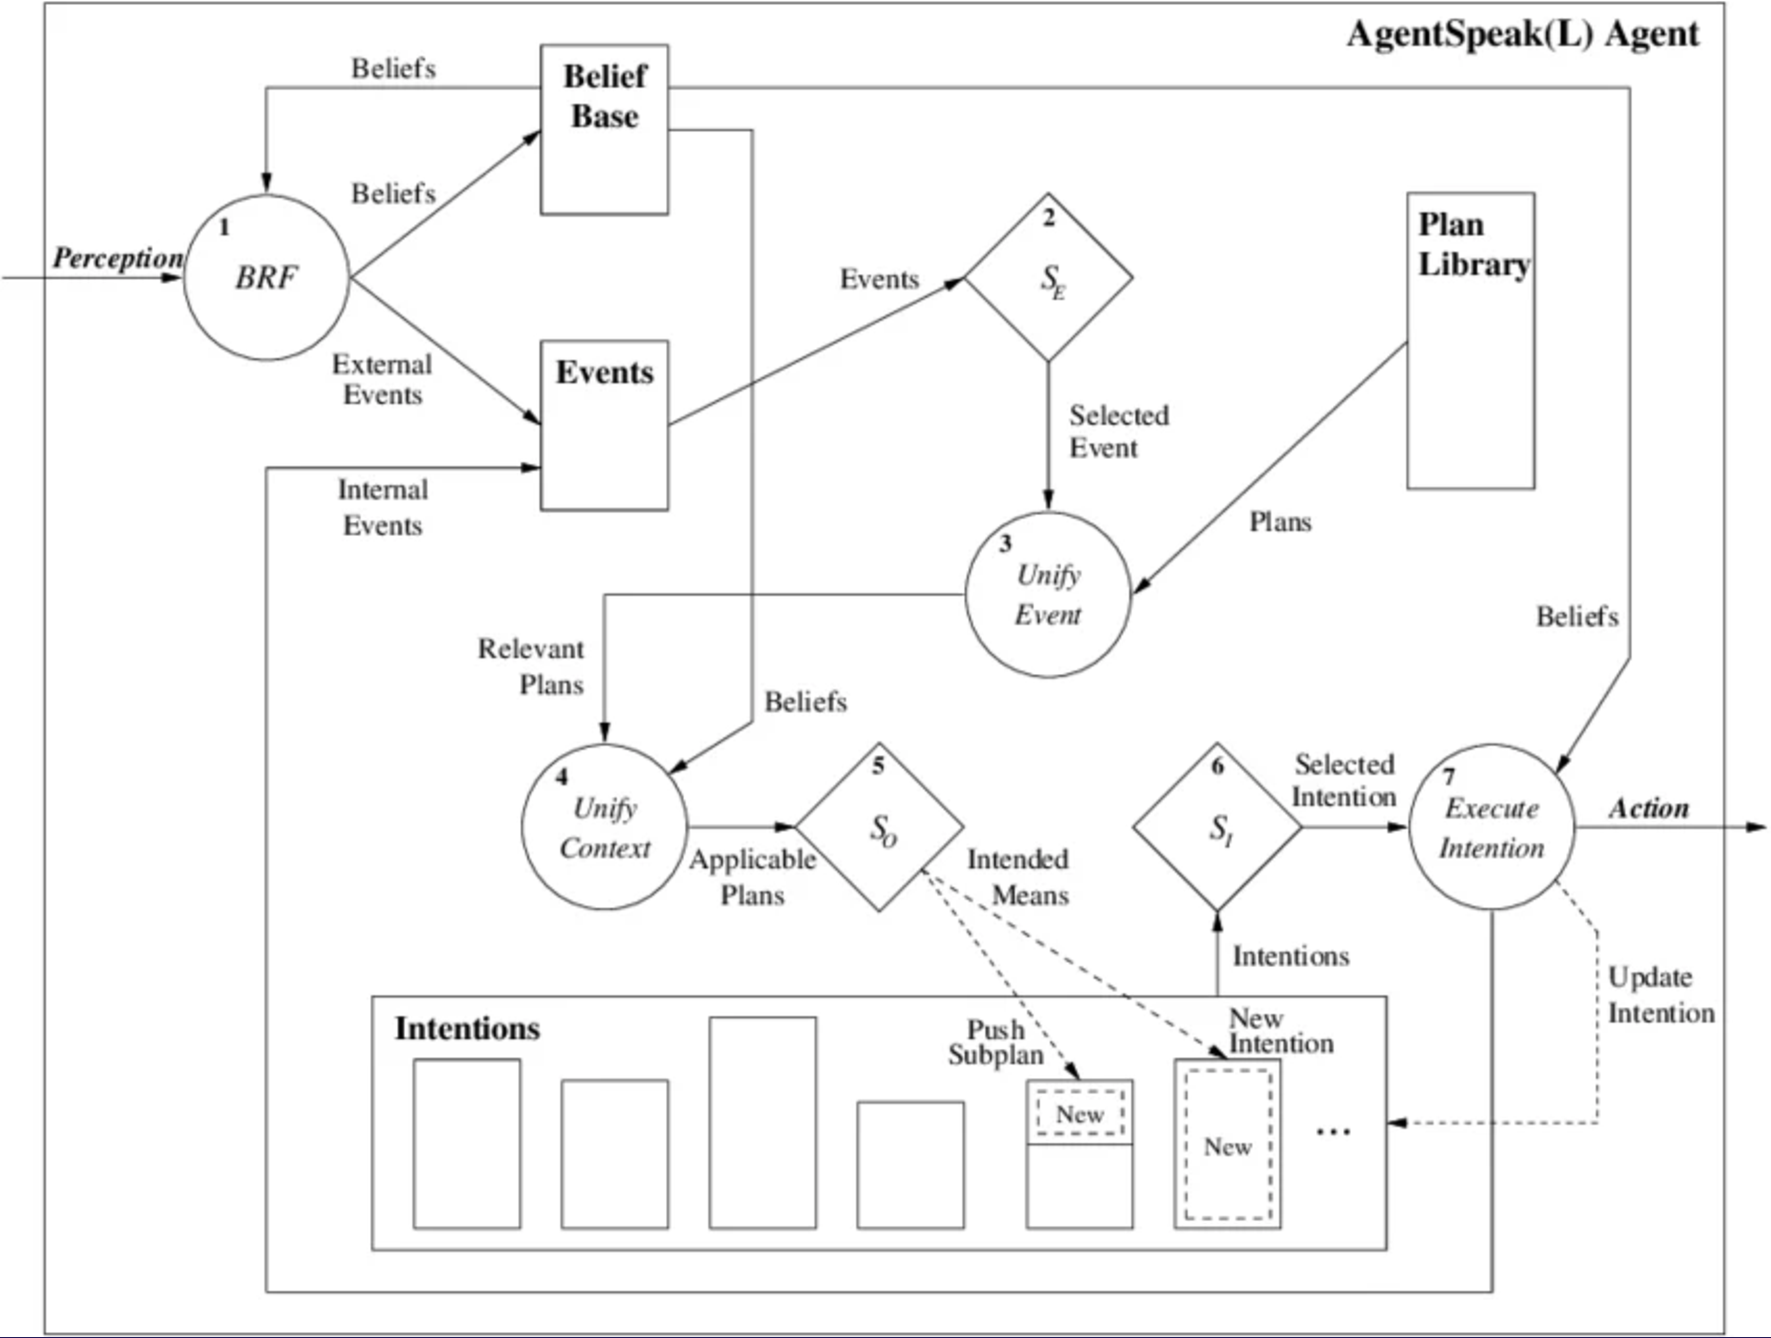
\includegraphics[width=0.8\textwidth]{figures/AgentSpeakL}
    \caption{AgentSpeak reasoning cycle. The figure illustrates the flow of the agent's reasoning process, from event selection to plan adoption and intention execution.}
    \label{fig:agentspeak}
\end{figure}

\paragraph{Beliefs}
Beliefs are represented as sets of ground terms and rules.
%
Rules are used to derive new knowledge from existing one,
where the predicate functor in the head of a rule defines the name of the belief.

\begin{lstlisting}[
    label=lst:belief,
    caption={
        \agentspeak{} belief representation as a logic rule. 
        %
        The rule states that X is the grandmother of Z if X is the mother of Y and Y is the parent of Z.
    },
    style=Prolog-cool
]
grandmother(X, Z) :- mother(X, Y), parent(Y, Z).
\end{lstlisting}

\Cref{lst:belief} is a representation of a belief in \agentspeak{}, 
where X, Y and Z are variables that can be instantiated with any value.
%
Predicates mother and parent assert whether a specific relationship holds between two entities, 
which can be true or false.
%
Following the example, 
grandmother belief is true only if X is the mother of some
Y and the same Y is the parent of Z.


\paragraph{Goals}
\agentspeak{} supports two types of goals that an agent can manage: \emph{achievement goals} and \emph{test goals}. 
%
Achievement goals represent a desired state of the world that the agent wants to achieve, 
which will eventually be reflected in its belief base. 
%
Test goals state that the agent wants to know whether a certain belief is acknowledged,
which will hold if the belief is present in the belief base.

\paragraph{Events}
All changes in the agent's mental state are represented as events,
whether they are triggered by the environment or by the agent's own reasoning process.
%
\agentspeak{} distinguishes between six types of events:
\begin{inlinelist}
    \item belief addition,
    \item belief removal,
    \item addition of an achievement goal,
    \item failure of an achievement goal,
    \item addition of a test goal,
    and
    \item failure of a test goal.
\end{inlinelist}

In AgentSpeak, events are represented using the notation $\langle op \rangle t$, 
where $op$ denotes the operation associated with the event 
and $t$ is the affected mental attitude, 
typically a belief or a goal. 
%
Conventionally, the operation is represented by the symbols $+$ and $-$,
which slightly change their meaning depending on whether they are applied to beliefs or goals.
%
In the case of beliefs,
the symbols $+$ and $-$ indicate the addition and deletion of a belief,
while in the case of goals,
they indicate the adoption and failure of a goal, respectively.

For example, the event $+b$ denotes the addition of the belief $b$ to the belief base, 
while $-b$ represents its removal. 
%
Similarly, $+!g$ denotes the adoption of an achievement goal $g$, 
whereas $+?g$ represents the request to verify whether the goal $g$ can be satisfied from the current belief base. 
%
These events are subsequently matched against the triggering events of plans, 
allowing the reasoning engine to identify the plans that are relevant to the current execution context.

\paragraph{Actions}
Primitive operations available to an agent
that can be used in plans to achieve its goals.
%
Examples of actions include sending messages to other agents,
performing operations on the environment,
or executing internal computations.
%
Actions are conceived as operations that are executed in a single lifecycle step,
and provide a mechanism for injecting the underlying language procedures and libraries into an agent's plans.

Pre-/post-conditions for an action are not explicitly represented in \agentspeak{}
as the actions are usually invoking low-level software/hardware facilities that bring side effects about.
%
In practice, 
\agentspeak{} actions are basically \emph{mnemonic names} of functionalities causing effects.
%
Typically,
in \ac{BDI} agents,
actions may even fail due to unpredictable environment dynamics making pre-/post-conditions hard to define.

\paragraph{Plans}
\agentspeak{} plans differ significantly from first-principles planning,
where the plan is a sequence of actions to be performed to reach a desired world state%
---i.e., \emph{declarative} goals~\cite{winikoff2002kr}.
%
\agentspeak{} plans are called \emph{plan rules} and have the form:
%
\inlineAsl{
E : C <- A$_1$; \ldots; A$_n$.
}
%
The rule specifies how the agent reacts to a \emph{triggering event} \inlineAsl{E},
for example when a new percept is received or when a goal must be achieved.
%
The \emph{context} \inlineAsl{C} contains the conditions that must hold for the rule to be applicable,
while \inlineAsl{A$_1$; \ldots; A$_n$} is the \emph{body}, i.e., the sequence of actions and sub-goals to execute.
%
A plan has a \emph{head} and a \emph{body}. The head includes the triggering event and the context, whereas the body contains the actions and goals to be performed.
%
A rule becomes relevant when its triggering event matches a current event, and it is selected only if the context is satisfied by the agent's belief base.
%
Once selected, the agent creates a new intention for that plan and schedules execution of its body over subsequent reasoning cycles.
%
The actions and sub-goals are then executed incrementally until the intention succeeds, suspends while waiting for sub-goals to be achieved, or is discarded.
%
Through the sub-goal mechanism,
\agentspeak{} agents can pursue complex goals by breaking them down into smaller sub-goals
for which the specific plans are selected at runtime,
resulting in a non-linear execution.

Although it is possible to write plans rules and goals in a declarative style to mimic classic planning~\cite{hubner2006dalt, HindriksBHM00},
it is often the case that a goal expressed as the triggering event
of a \ac{BDI} plan rule
is simply a \emph{mnemonic name} of an event the agent may react to%
---i.e., \emph{procedural} goals~\cite{winikoff2002kr}.

\begin{lstlisting}[
    label=lst:plan,
    caption={
        \agentspeak{} definition for plans.
        %
        The plan is triggered by the addition of a belief about the presence of waste at a given location in the environment.
        %
        The plan is applicable only if the robot is already located at that position, and whether the robot knows the position of the bin.
        %
        If selected, the plan executes a sequence of actions: the robot first picks up the waste, then triggers the plan that moves the agent to the location of the waste bin, and finally deposits the collected waste into the bin.
    },
    style=Prolog-cool
]
+location(waste, X) : location(robot, X) & location(bin, Y)
                    <- pick(waste);
                       !location(robot, Y);
                       drop(waste).
\end{lstlisting}

An example of an AgentSpeak plan is reported in \Cref{lst:plan}, 
describing the behaviour of a robot responsible for waste collection. 
%
The highlighted plan is triggered when waste is detected at a given location \prologInline{X} in the environment. 
%
The plan is applicable only if the robot is already located at that position, 
and if the robot knows the position of the waste bin \prologInline{Y}. 
%
When selected, 
the plan executes a sequence of actions: 
the robot first picks up the waste, 
then triggers the achievement goal that moves the robot to the location of the waste bin, 
and finally deposits the collected waste into the bin. 
%
Naturally, 
the robot must also possess additional plans enabling it to navigate to the required locations, 
so that the sub-goal invoked by the plan can be successfully accomplished.

%
The underlying \agentspeak{} assumption is that all plans are known in advance,
and the agent can select them based on the current context.
%
Then,
it may happen that a plan is not available for a given event and context,
in which case the agent may fail to achieve the goal.
%
To make that possible,
\agentspeak{} assumes that low-level software/hardware facilities are attached to the agent,
and that executing the action will invoke them accordingly.
%

\subsection{Recent Extensions of \agentspeak{}}

Although \agentspeak{} core abstractions 
have remained substantially unchanged since their original formulation,
the framework continues to attract significant research interest. 
%
Rather than replacing its symbolic foundations, 
recent work extends the language to address new \emph{software engineering} challenges, improve agent \emph{organization}, and integrate modern \emph{artificial intelligence} techniques. 

\paragraph{Software Engineering}
\agentspeak{} initial definition offers limited support for developing large-scale and reusable software systems. 
%
Consequently, 
some extensions introduced programming abstractions aimed at improving modularity, 
encapsulation, 
and code reuse.
%
An effort towards modularity is presented in~\cite{agentspeak-extension-modularity}, 
where plan libraries can be imported from external source files, 
allowing plans to be shared across multiple agents and applications. 
%
This mechanism promotes software reuse 
while preserving the original \agentspeak{} syntax.
%
Further improvements have been proposed in AgentSpeak(ER)~\cite{ricci2018atal}, 
which extends the language with mechanisms for structuring reactive behaviour. 
%
In particular, 
reactive plans can be defined within the body of other plans, 
enabling developers to organise complex behaviours hierarchically and to encapsulate reactive functionalities within higher-level plans.
%
\ac{OOP} principles inspired some \agentspeak{} extensions. 
%
For instance, 
\cite{croatti2016agere} introduces scoped beliefs in addition to reactive plans, 
allowing beliefs to be encapsulated within a specific plan or agent. 
%
This improves information hiding and facilitates the development of modular agent specifications. 
%
Similarly, 
\cite{agentspeak-extension-collier} propose an inheritance mechanism for \agentspeak{} agents, 
enabling developers to define reusable agent specifications that can be extended and specialized to implement new agent types. 
%
Collectively, 
these works demonstrate a common effort towards enriching \agentspeak{} with software engineering abstractions while preserving its original cognitive and declarative foundations.


\paragraph{Organizational and social reasoning}
Many real-world multi-agent systems 
require agents to operate within organizations, 
where their behaviour is regulated by 
roles, 
norms, 
obligations, 
permissions, 
and institutional rules. 
%
However, 
the original \agentspeak{} language 
provides no native abstractions 
for representing or reasoning about such organizational concepts.
%
To address these requirements, 
some extensions extensions enrich 
the \agentspeak{} reasoning process 
with organizational and normative concepts.
%
AgentSpeak(RT)~\cite{agentspeak-rt}, 
for instance, 
extends intentions with \emph{deadlines}, 
specifying the time by which an agent should respond to an event, 
and \emph{priorities}, 
defining the relative importance of responding to competing events. 
%
These additions enable the reasoning cycle 
to take temporal constraints and event priorities into account 
during deliberation.
%
Building upon these ideas, 
N-Jason~\cite{N-Jason} extends AgentSpeak(RT) 
with explicit normative abstractions, including 
obligations, 
permissions, 
prohibitions, 
deadlines, 
priorities, 
and durations. 
%
In addition to extending the language syntax, 
N-Jason modifies the operational semantics by introducing norm-aware deliberation into the reasoning cycle. 
%
In particular, it adds two additional stages: 
\emph{event reconsideration}, 
in which the agent analyses the objectives associated with the applicable norms, 
and \emph{option reconsideration}, 
where the agent evaluates the available plans to determine the most appropriate response while taking normative constraints into account.

More recently, 
research has explored the introduction of organizational roles 
as first-class language abstractions. 
%
In~\cite{dynamic-roles-agentspeak}, 
roles can be dynamically acquired, 
relinquished, 
or transferred during execution, 
allowing agents to adapt their behaviour according to the organizational context in which they operate. 
%
Unlike the original \agentspeak{} semantics, 
where plan applicability depends exclusively on triggering events and belief contexts, 
role-aware extensions incorporate the agent's role into 
the deliberation process, 
enabling more flexible coordination and dynamic reorganization within multi-agent systems.

Collectively, 
these proposals extend the original cognitive model of \agentspeak{} with explicit representations of social and organizational concepts. 
%
Rather than modifying the fundamental \ac{BDI} abstractions, 
they enrich the reasoning process with additional information that enables agents to reason not only about the organizational context in which they operate.


\paragraph{Integration with generative artificial intelligence}

The recent success of large language models has opened a new research direction for \agentspeak{-based} systems. Traditionally, an agent's plan library is statically defined by the developer before execution. 
%
Although this is beneficial for the agent's predictability and controllability,
it limits the agent's flexibility and adaptability to unforeseen situations.
%
For this reason,
the \ac{BDI} community has long been interested in the problem of \emph{automatic plan generation},
incorporating techniques from \ac{AI} planning into the \ac{BDI} architecture.
%
The objective is to combine the adaptability and generative capabilities with the symbolic reasoning, 
explicit knowledge representation, 
and execution transparency offered by \agentspeak{}. 

Several approaches explore combining \acp{BDI} principles with \acp{LLM},
rather than focusing on the integration of generative capabilities
into the well-established \agentspeak{}-based architecture
%
The work by \cite{IchidaM024} proposes NatBDI,
a \ac{BDI} agent architecture designed for natural language environments.
%
It leverages \acp{LLM},
specifically for \ac{NLI},
within the \ac{BDI} reasoning cycle to determine the applicability of plans based on natural language beliefs and context descriptions,
rather than generating the plans themselves.
%
Another direction, presented by \cite{JangYCO023},
uses the \ac{BDI} structure itself to create structured prompts (``BDIPrompting'') for \acp{LLM}.
%
This guides the \ac{LLM} to generate more proactive and explainable task plans
by framing the planning problem in terms of beliefs, desires, and intentions
directly within the prompt given to the \ac{LLM}.
%
Another interesting approach is \cite{2025chatbdi},
which involves \acp{LLM} to enhance conversation capabilities between \ac{BDI} agents and humans.

\paragraph{Open challenges}

Despite nearly three decades of research, several challenges remain open. 
%
Current \agentspeak{} technologies still exhibit limitations with respect to interoperability, modular software development, concurrency management, debugging support, and verification. 
%
Moreover, while recent advances in generative artificial intelligence significantly extend the applicability of the language, 
integrating these capabilities without compromising the formal semantics of \agentspeak{} remains an active area of investigation.
%
Traditional \ac{BDI} programming frameworks typically lack mechanisms allowing agents to autonomously acquire
or build new plans at runtime~\cite{SilvaSP09}.
%
The procedural behaviour of \agentspeak{} agents is then limited
to scenarios where the agent behaviour can be suitably defined at design time (pre-programmed):
an effective option in terms of computational efficiency,
which however constrains agent flexibility, responsiveness, and overall \emph{autonomy} when facing unpredictable environments.

Overall, recent research demonstrates that \agentspeak{} continues to evolve through extensions that preserve its original symbolic and declarative foundations 
while expanding its applicability to increasingly complex and heterogeneous software systems. 

\subsection{\agentspeak{} Frameworks}
\label{subsec:agentspeak-frameworks}

Although \agentspeak{} provides a well-defined operational semantics for programming \ac{BDI} agents, 
it does not prescribe a specific software implementation. 
%
Consequently, since its introduction, 
the research community has proposed numerous programming languages and frameworks inspired by, 
or directly implementing, 
the \agentspeak{} semantics. 
%
While these technologies share the same cognitive foundations, 
they differ considerably in terms of language design, 
execution platforms, 
interoperability mechanisms, 
software engineering support, 
and runtime characteristics.

Rather than providing a comprehensive survey of every \agentspeak{}-inspired technology proposed in the literature, 
this section focuses on frameworks that satisfy two criteria. 
%
First, they provide an actively maintained implementation of the \agentspeak{} programming model. 
%
Second, they are intended for the development of general-purpose \ac{BDI} agents, 
rather than targeting specific application domains.
%
Accordingly, 
this comparison builds upon the survey by Calegari \textit{et al.}~\cite{lptech4mas-jaamas35}, 
which reviews the state of the art of logic-based agent-oriented technologies. 
%
As far as \ac{BDI} agent programming languages are concerned,
the comparison focuses on those languages that appear to have some running software implementation
that is actively maintained and used by the community.
%
For completeness, 
we also include \jakta{} in the comparison, 
although its development postdates the analysis of the other frameworks. 
%
The rationale behind the design choices adopted in \jakta{} is discussed in Section~\ref{sec:jaktadsl}.

The comparison is not intended to establish a ranking among the considered technologies. 
%
Instead, its objective is to identify the design choices adopted by existing \agentspeak{} implementations, 
highlighting both their strengths and their limitations from a software engineering perspective. 
%
% These observations motivate several of the architectural decisions underlying the design of \jakta{}.

Table~\ref{tab:languages-comparison} summarizes the comparison, 
while the remainder of this subsection discusses the considered dimensions in detail:
\begin{itemize}
    \item full \textbf{\agentspeak{} compliance};
    %\item \textbf{logic programming} support, i.e. the capability to rely upon the mechanisms of unification and backtracking to represent and manipulate \ac{BDI} data structures;
    \item \textbf{\ac{DSL} type} (internal or external);
    \item \textbf{hosting syntax}, i.e., which syntax the \ac{DSL} is embedded in (for internal \acp{DSL}) or based upon (for external \acp{DSL});
    \item \textbf{execution platform}, i.e., which runtime platform the language runs upon;
    \item \textbf{interoperability}, i.e., whether and how other languages can be called from within the \ac{BDI} language (and, in that case, which ones);
    \item \textbf{paradigm blending}, i.e., whether it is possible to mix, in the same source and scope, AOP and other abstractions;
%        (for instance, creating objects inside plans and treating plans as objects);
    \item \textbf{type safety}, i.e., the ability of the compiler/interpreter to intercept (most) type errors ahead-of-execution;
    \item \textbf{reuse mechanisms}, i.e., whether and how it is possible to parameterise and reuse partial or entire \ac{MAS} specifications;
    \item \textbf{concurrency model} i.e., whether the \ac{MAS} platform supports developers in switching between multiple ways to execute agents;
    \item \textbf{explicit environment}, i.e., whether the language provides it as an explicit \emph{and} programmable abstraction;
    \item \textbf{internal actions}, namely, whether the language provides mechanisms to implement agent introspection
          (i.e., observing the agent's own state) and related reasoning;
    \item \textbf{external actions}, akin to internal actions, but related to the perception of and actuation over the environment;
    \item \textbf{message-passing mechanism}, i.e., how inter-communication among agents is actually supported;
    and, finally,
    \item \textbf{license}, which can impact severely on the adoption of a technology.
\end{itemize}

% !TeX root = ../paper-2024-sncs-jakta.tex
\begin{landscape}
% GC: ho messo landscape perché adjustbox non funziona
\begin{table}
    \footnotesize
%    \begin{adjustbox}{max width=\textwidth}
    \begin{tabular}{r||c||c|c|c|c|c|c|c}
    \textbf{} &
      \textbf{\makecell[c]{\jakta\\\cite{DBLP:journals/sncs/BaiardiBCP24}}} &
      \textbf{\makecell[c]{\jason\\\cite{BordiniHW2007}}} &
      \textbf{\makecell[c]{\spadebdi\\\cite{PalancaRCJT22}}} &
      \textbf{\makecell[c]{\phidias\\\cite{DUrsoLS19}}} &
      \textbf{\makecell[c]{\astra\\\cite{CollierRL15}}} &
      \textbf{\makecell[c]{\jack\\\cite{Winikoff2005}}} &
      \textbf{\makecell[c]{\jadex\\\cite{PokahrBL2005}}} &
      \textbf{\makecell[c]{\goal\\\cite{Hindriks2009}}}
      \\\hline\hline
    \textbf{\makecell[r]{AgentSpeak\\compliance}} &
      \yes &
      \yes &
      \yes &
      \yes &
      \no &
      \no &
      \no &
      \no
      \\\hline
    \textbf{DSL Type} &
      internal &
      external &
      both &
      internal &
      external &
      external &
      external &
      external
      \\\hline
    \textbf{\makecell[r]{Hosting\\Syntax}} &
      Kotlin &
      \makecell{AgentSpeak\\extension} &
      Python &
      Python &
      \makecell{Java\\extension} &  % astra
      \makecell{Java\\extension} &  % jack
      \makecell{XML, Java\\annotations} &  % jadex
      \makecell{Prolog\\extension}  % goal
      \\\hline
    \textbf{\makecell[r]{Execution\\Platform}} &
      JVM &
      JVM &
      Python &
      Python &
      JVM &
      JVM &
      JVM &
      \makecell{JVM}
      \\\hline
    \textbf{Interop.} &
      \makecell[c]{native Java\\and Kotlin,\\FFI native} &
      \makecell[c]{FFI Java} &
      \makecell[c]{native\\Python,\\FFI native} &
      \makecell[c]{native\\Python,\\FFI native} &
      \makecell[c]{FFI Java} &
      \makecell[c]{FFI Java} &
      \makecell[c]{FFI Java} &
      \makecell[c]{native\\SWI-Prolog}
      \\\hline
    \textbf{\makecell[r]{Paradigm\\blending}} &
      \yes &
      \no &
      \yes &
      \yes &
      \yes &
      \yes &
      \no &
      \yes
      \\\hline
    \textbf{Type safety} &
      \yes &
      \no &
      \no &
      \no &
      \yes &
      \yes &
      \yes &
      \no
      \\\hline
    \textbf{\makecell[r]{Reuse\\mechanisms}} &
      \makecell{Any Kotlin\\mechanism} &
      \makecell{file incl.,\\int. actions} &
      \makecell{Any\\Python\\mech.} &
      \makecell{Any\\Python\\mech.} &
      \makecell{agent\\extension} &
      \makecell{reusable\\plans and\\capabilities} &
      \makecell{file incl., Java\\inheritance} &
      \makecell{reusable\\plans, beliefs,\\goals, agents}
      \\\hline
     \textbf{\makecell[r]{Concurrency\\Model conf.}} &
    %  Pluggable &
    %  \makecell{One thread\\ per agent} &
    %  \makecell{Python\\ coroutines} &
    %  \makecell{One thread\\ per agent} &
    %  \makecell{One thread\\ per intention} &
     \yes &
     \yes &
     \no &
     \no &
     \yes &
     \dunno &
     \yes &
     \yes
     \\\hline
    \textbf{\makecell[r]{Explicit\\Environment}} &
      \yes &
      \yes &
      \no &
      \no &
      \yes &
      \no &
      \no &
      \yes
      \\\hline
    \textbf{\makecell[r]{Internal\\Actions}} &
      \yes &
      \yes &
      \yes &
      \yes &
      \yes &
      \no &
      \no &
      \yes
      \\\hline
    \textbf{\makecell[r]{External\\Actions}} &
      \yes &
      \yes &
      \no &
      \no &
      \yes &
      \no &
      \no &
      \yes
      \\\hline
   \textbf{\makecell[r]{Message\\Passing}} &
     pluggable &
     pluggable &
     XMPP &
     \makecell{HTTP \\ TCP Sock.} &
     UDP &
     pluggable &
     TCP / SSL &
     in process
     \\\hline
    \textbf{License} &
      Apache 2.0 &
      LGPL v3 &
      GPL v3 &
      MIT &
      GPL v3 &
      Proprietary &
      GPL v3 &
      GPL v3
    \end{tabular}%
%    \end{adjustbox}
    % \begin{center}\tiny
    %     * \jason{} supports plugging custom external actions by overriding a method on the environment class of choice.
    % \end{center}
    \normalsize
    \bigskip
    \caption{
        Comparison of the identified practical features across several common \ac{BDI} agent programming languages.
        Columns denote languages, rows denote features.
        \jakta{} is the language proposed in this paper: it is reported here for to ease comparison.
        In non-textual cells, symbol \yes{} indicates the feature availability,
        \no{} unavailability,
        and % ``\maybe'' means uncertainty, and
        \dunno{} that we were not able to find conclusive evidence.
    }
    \label{tab:languages-comparison}
  \end{table}
\end{landscape} 

\paragraph{Full \agentspeak{} compliance}

We distinguish between fully compliant \ac{BDI} technologies 
and the ones that are just inspired to \agentspeak{}.
%
Since such compliance,
to the best of our knowledge,
has not yet been formally defined,
for the scope of this section we rely on the following set of necessary features:
%
\begin{enumerate}
    \item explicit representation of beliefs, goals, plans, and events in the language syntax;
    \item explicit representation of belief bases, events, plan libraries, and intentions in the engine;
    \item all the aforementioned representations are based on logic terms and clauses,
    thus including:
    %
    \begin{enumerate}
        \item arbitrarily structured, possibly nested and non-ground, logic terms and clauses;
        \item logic unification and resolution (cf. \cite{KornerLBCDHMWDA22})
        to manipulate the aforementioned data structures;
    \end{enumerate}
    \item event-based architecture for the execution of the reasoning cycle;
    \item explicit support for (at least) achievement and test goals.
\end{enumerate}

Our analysis identified that both \jason{} and \spadebdi{} are fully compliant to the \agentspeak{} definition,
in fact, they both can describe agents by the means of \kotlinInline{.asl} files,
which are structured to represent beliefs, goals, plans, and events following the abstract semantics of \agentspeak{}.
%
Furthermore, \phidias{} adheres to our definition of \agentspeak{} compliance as well,
even though it does not support the \agentspeak{} syntax directly,
as they come with an internal domain-specific language.
%
\goal{} supports logic representation,
but is missing intentions and test goals,
hence we classify it as not fully compliant.
%
Similarly, even though \astra{} supports all the \agentspeak{} features,
it does not fully support logic programming to represent beliefs, goals, plans, and events.
%
\jadex{} does not provide any unification mechanism.
%
Finally,
although \jack{} explicitly models beliefs and plans,
it does not represent them using logic terms;
rather, its \textit{beliefs sets} work as in-memory relational databases.
%
Thus, we classify \jack{} as not \agentspeak{}-compliant.

\paragraph{\ac{DSL} type and hosting syntax}

The former feature categorizes \ac{BDI} languages as either \emph{external} or \emph{internal} \ac{DSL}, or possibly both of them.
%
Conversely, the latter feature provides further details about the \ac{DSL} syntax.
%
The two features are strictly related, as they both refer to the syntax of the language.
%
In fact, for internal \acp{DSL},
one may be interested in understanding which syntax the \ac{DSL} is embedded in,
whereas, for external \acp{DSL}, we further describe the derivation of the syntax.
%
Accordingly, regarding internal \acp{DSL},
both \spadebdi{} and \phidias{} are hosted by Python.
%
Conversely, the syntax of external \acp{DSL} is built as an extension or refinement of a \ac{GPL}.
%
For instance, while \jadex{} relies on XML,
\goal{} extends Prolog~\cite{KornerLBCDHMWDA22}, and \jason{} extends \agentspeak{}; whereas \astra{} and \jack{} extend Java.

\paragraph{Execution platform}

The execution platform is the runtime environment which is required for running a given \ac{BDI} language---as well as the \ac{MAS} described through it.
%
It is worth highlighting that several programming languages may be executed on the same platform.
%
This is the case,
for instance,
in Kotlin, Java, and Scala which are all executed on the \ac{JVM} platform.
%
The execution platform is a relevant feature, as it may affect the portability of the \ac{MAS},
as well as its interoperability with other systems and languages.
%
Considering the languages under comparison,
\spadebdi{} and \phidias{} target Python,
while all the other ones target the \ac{JVM}.

\paragraph{Interoperability}
%
This feature concerns the ability of the agent programming language to interact with the host language constructs.
%
Interaction can be achieved in three different ways:
\begin{enumerate}
    \item \emph{native}: the \ac{AOP} language is capable of directly calling the \ac{GPL} language constructs;
    \item \emph{\ac{FFI}}: the \ac{AOP} language features a dedicated \ac{API} allowing streamlined interaction;
    \item \emph{indirect}: communication is possible, but it requires manually concocted workarounds
        (e.g., communication via sockets or files).
\end{enumerate}
%
We consider in this discussion only the two former types of interoperability.
%
Internal \acp{DSL} such as \phidias{} and \spadebdi{} are capable of native interoperability by constructions
(they are valid fragments in the host \ac{GPL}),
while external \acp{DSL} require, typically, the use of a \ac{FFI}.
%Specifically, this feature is about which other languages the \ac{BDI} language at hand can directly call, exploiting the hosting language interoperability mechanisms.
%
All the languages targeting the \ac{JVM} we considered can interoperate with Java constructs,
but in many cases this interaction must be carefully crafted, adapting to an existing API,
which may require the creation of glue code.
%
For instance,
in Jason the programmer must adhere to pre-defined Java interfaces provided by the framework,
producing pure Java code that can then get called from Jason.
%
Once Java interoperability is established,
it is often possible to call also other \ac{JVM} languages
(Scala, Kotlin, Groovy, etc.),
limited to the fragments that produce bytecode overlapping Java's\footnote{
    Producing fully-Java-interoperable bytecode from languages targeting the JVM other than Java is often possible,
    but it requires special care.
    %
    For instance,
    Kotlin recommends using annotations to explicitly define how Kotlin constructs should be translated into Java ones,
    see the Kotlin's documentation on ``Calling Kotlin from Java''
    archived at \url{https://archive.is/HqEIG}.
    %
    Scala features many mechanisms that are not directly translatable into Java,
    such as implicits, higher-kinded types, mixins, and multiple argument lists.
    %
    The official compatibility guide provides only general information on cross-compatibility
    (see the archived documentation about ``Interacting with Java'' at \url{https://archive.is/KX49E});
    however,
    compatibility guides are available from third parties such as Databricks,
    which recommends not using several Scala features in order to make the code compatible
    (see the ``Java interoperability'' section of the guide archived at \url{https://archive.ph/Qc9Gd}).
    %
    For even more conceptually distant languages such as Clojure,
    the operation may be borderline impossible:
    according to the official documentation archived at \url{https://archive.is/AeNcE},
    Interoperability requires the use of a dedicated Clojure \ac{FFI} library.
    %
    The take-away message is that native or \ac{FFI}-based interoperability with Java
    does not automatically imply interoperability with other \ac{JVM} languages.
}.
%
However,
notice that the presence of a \ac{FFI} does not tell the entire story about \emph{ease} of interoperability.
%
For instance,
although implemented in Java,
\jadex{} requires the \ac{MAS} specification to be written in XML,
making interoperability with Java code cumbersome
compared to other \ac{JVM}-based \ac{AOP} languages.

\paragraph{Paradigm blending}
%
We call paradigm blending the \emph{syntactical} language capability to mix,
in the same code fragment,
\ac{AOP} constructs and \ac{GPL}-native constructs implementing a different paradigm's abstractions,
such as object creation and manipulation (for \ac{OOP} languages)
or higher-order functions definition and invocation (for \ac{FP} languages).

Notice that whether blending is beneficial or detrimental depends on the goal of the language.
%
As a rule of thumb,
blending tends to be beneficial when building complex applications,
of which different parts may be better expressed in different paradigms.
%
On the other hand,
it may be a double-edged sword when \emph{learning} a new paradigm,
as the inexperienced may be tempted to work around problems more easily tackled with \ac{AOP} using other paradigms they feel more comfortable with.
%
Notice, in fact,
that some languages purposely enforce a clear separation among high-level AOP constructs
(e.g., belief, goals, plans)
and the hosting language ones (e.g. classes, functions, etc.),
purposely allowing interoperation only through carefully-crafted \acp{FFI}~\cite{DBLP:conf/eumas/BergentiMP23}.
%
The strong separation is typical of
\jason{} and \jadex{}.
%
There, in the former case, \acp{MAS} are composed by scripts describing agent specifications
supporting solely \agentspeak{}-compliant constructs,
and, in the latter, by actions/environment written in ordinary Java.

Interestingly,
languages whose syntax is blended with the hosting language may be further categorized into two sub-sorts,
depending on whether they
%
\begin{inlinelist}
    \item\label{case:aop-into-oop}
    limit the use of the \ac{GPL}'s abstractions into agents/plans specifications, or
    \item\label{case:oop-into-aop} allow the \ac{GPL}'s constructs to appear into \ac{AOP} programs directly.
\end{inlinelist}
%
Case~\ref{case:aop-into-oop}, for instance,
characterizes Python-based \ac{BDI} languages such as \spadebdi{} and \phidias{},
where AOP specifications consist of Python classes and methods.
%
Conversely, \astra{}, \jack{}, and \goal{} adopt strategy~\ref{case:oop-into-aop},
as their syntaxes permit writing Java or Prolog constructs and libraries, respectively.

\paragraph{Type safety}
%
This feature refers to the presence of a strict compile-time type checker for the \ac{BDI} language at hand,
which may proof check agents specifications before execution.

Solutions featuring tight interoperability with Java,
such as \astra{}, \jack{}, and \jadex,
come with this feature;
whereas the other languages in this comparison do not.
%
Those (\jason{}, \spadebdi{}, \phidias{}, and \goal{})
favour a flexible syntax over type safety,
as they rely on weakly-typed hosting languages such as Prolog or Python.

\paragraph{Reuse mechanisms}
%
This feature refers the presence of abstraction mechanisms supporting the reuse of partial \ac{MAS} specifications.
As far as this feature is concerned, we observe great variety among the surveyed languages.
%
Some rely on bare file inclusion mechanisms.
%
This is the case, for instance,
of \jason{},
supporting the inclusion of ASL files into other ASL files;
and \jadex{},
which, in addition to Java inheritance between agent classes,
supports referencing XML or Java files into other XML files for more flexible reuse of agents' capabilities.

Furthermore, virtually all surveyed solutions support the abstraction and reuse mechanisms of the hosting language, if any.
%
For instance,
internal actions in \jason{} are defined as
pure Java classes,
thus they can be reused across multiple projects.
%
This implies,
for instance,
that solutions based on a \ac{OOP} host \ac{GPL} may take advantage of its \ac{OOP} abstraction mechanisms,
such as sub-typing and inheritance,
for the \ac{OOP}-written portions of their \ac{MAS} specifications.

Some solutions may also expose high-level, agent-oriented notions -- such as agents or plans -- as first-class syntactical constructs.
%
In other words, they may provide ad-hoc syntax for writing agents or plans.
%
This is the case, for instance, of \astra{}, \jack{}, and \goal{}.
%
When this is the case,
first-class abstraction can be reused along the \ac{MAS} specification.
%
For example,
\astra{} supports writing agents' specifications extending other agents' specifications,
whereas \jack{} bases its modularity on the concept of capabilities~\cite{busetta1999structuring} wrapping beliefs and plans.

\paragraph{Concurrency model}

This feature is about how the surveyed solutions deal with agents' \emph{concurrent execution},
and whether developers can select among multiple execution models
without resorting to changes in the execution platform's code.
%
Despite agents having their own \emph{logical} control flow -- as required by their computational autonomy --,
how such control flow is mapped in practice over processes, threads, and other platform- and operating system-specific concurrency facilities may vary wildly.
%
The mapping between logical and physical control flows may affect several runtime properties of a \ac{MAS}:
performance and scalability are the most obvious one,
but also determinism and
reproducibility
(hence, testability) are deeply affected.

Admissible choices in this case are manifold.
%
The most common ones are:
%
\begin{description}
    \item[\ac{1A1T}] where each agent is mapped over a single thread;
    \item[\ac{AA1T}] where all agents in the system share the same thread;
    \item[\ac{AA1E}] where all agents in the system share the same executor service;
    \item[\ac{1A1P}] where each agent is mapped over a single process.
\end{description}

\jason{}, \astra{}, \jadex{} and \goal{} provide mechanisms that allow developers to customise execution strategies for their \ac{MAS}.
%
They provide support for multiple strategies out of the box
(of which one,  \acs{AA1E} is set as default),
and they provide \acp{API} to regulate the amount of threads in the executor.

\phidias{},
instead, is hard-coded to \acs{1A1T}.
%
\spadebdi{},
relying on Python coroutines that are single-threaded by default\footnotemark,
implicitly adopt the \acs{AA1T} model.
\footnotetext{Developing with \texttt{asyncio}, Concurrency and Multithreading, Python 3 docs. Archived at \url{https://archive.is/YWQw5}}
%
In the case of \jack{},
the documentation does not discuss the available concurrency abstractions,
nor it explains how to select them or provide a custom one.


\paragraph{Explicit environment}
%
The design of environments
is essential for multi-agent systems that rely on stigmergy~\cite{weyns2007aamas}.
%
We analyse whether the \ac{BDI} languages under scrutiny feature an explicit and \emph{programmable} notion of environment.
%
To the best of our knowledge,
the environment is modelled as a first-class programmable construct in \jason{}, \astra{}, \goal{}.

\paragraph{Internal/External actions support}
%
This feature is about whether \ac{BDI} languages come with some means to enrich agents' or environments' specifications
with custom functionalities written via the host language.
%
Using \jason{}'s nomenclature, we call these functionalities ``external (resp. internal) actions'',
if they extend the agents' capability to perceive/affect the environment (resp. their own internal state).
%
From a programming language perspective, actions are the technical bridge between the agent- and the object-oriented portions of a \ac{MAS} specification.

The support for internal or external actions is heterogeneous among \ac{BDI} languages (cf. \Cref{tab:languages-comparison}),
and we identified that \jason{}, \astra{}, and \goal{} support both of them.
%
For those languages for which we did not identify an explicit notion of environment,
we assumed that the mechanism of external actions is not supported as well.
%
Neither \jack{} nor \jadex{} provide first-level abstractions for actions,
instead, both provide customisation mechanisms,
the first one through the concept of ``capability''~\cite{busetta1999structuring},
while the second leveraging Java inheritance.

\paragraph{Message passing mechanism}
%
Despite most \ac{BDI} languages coming with primitives enabling agent interaction via message-passing,
they may differ in the way they support message exchange in practice.
%
This feature is about \emph{how} \ac{BDI} languages support message exchange.
%
Options involve:
%
\begin{inlinelist}
   \item\label{case:in-process} in-process communication,
   enabling communication only among agents sharing the same runtime;
   \item\label{case:distributed} distributed communication,
   possibly involving data exchanges over networked machines;
   and
   \item\label{case:pluggable} customisable communication,
   in which, both the previous cases can be supported, depending on the configuration.
\end{inlinelist}

Case~\ref{case:in-process} is native in \goal{}~\cite{Hindriks2009}.
%
Conversely,
\spadebdi{}, \astra{}, \phidias{} and \jadex{} are characterized by case~\ref{case:distributed},
as they rely upon the XMPP, UDP, TCP sockets or HTTP, and TCP/SSL protocols respectively.
%
\jason{} and \jack{}~\cite{Winikoff2005} fall into Case~\ref{case:pluggable}.

\paragraph{License}
%
This feature is about which license \ac{BDI} solutions are distributed with,
which is crucial for the adoption of the technology.
%
Mainly,
solutions can require a fee for their usage,
being free of charge but not open source,
or being open source
(hence, inspectable and extendable).
%
All solutions but \jack{} (which is proprietary, commercial, and closed-source) adopt a \ac{FOSS} license.

\section{\acl{AC}}
\subsection{Macroprogramming}
\subsection{\acl{AC}}
\subsection{\acl{AC} Frameworks}
